
\documentclass[runningheads,a4paper]{llncs}

\usepackage{amssymb}
\setcounter{tocdepth}{3}
\usepackage{graphicx}

\usepackage{url}
\urldef{\mailsa}\path|{ismael.rivera, knud.moeller}@deri.org| 
\urldef{\mailsb}\path|zuendorf@cs.uni-kassel.de|
%\urldef{\mailsc}\path|erika.siebert-cole, peter.strasser, lncs}@springer.com|    
\newcommand{\keywords}[1]{\par\addvspace\baselineskip
\noindent\keywordname\enspace\ignorespaces#1}

\usepackage{amssymb}

\newenvironment{listing}
{\begin{list}{}{\setlength{\leftmargin}{1em}}\item\scriptsize\bfseries}
{\end{list}}

\begin{document}

\mainmatter  % start of an individual contribution

% first the title is needed
\title{An improved platform for Web service wrapping, discovery and consumption}

% a short form should be given in case it is too long for the running head
\titlerunning{Enhancing the discovery and consumption of Web services}

% the name(s) of the author(s) follow(s) next
%
% NB: Chinese authors should write their first names(s) in front of
% their surnames. This ensures that the names appear correctly in
% the running heads and the author index.
%
\author{Ismael Rivera\and Knud M\"oller\and Albert Z\"undorf}
%
\authorrunning{Ismael Rivera\and Knud M\"oller\and Albert Z\"undorf}
% (feature abused for this document to repeat the title also on left hand pages)

% the affiliations are given next; don't give your e-mail address
% unless you accept that it will be published
\institute{DERI, National University of Ireland, Galway\\
University of Kassel, Germany\\
\mailsa\\
\mailsb\\
%\mailsc\\
%\url{http://www.springer.com/lncs}
}

%
% NB: a more complex sample for affiliations and the mapping to the
% corresponding authors can be found in the file "llncs.dem"
% (search for the string "\mainmatter" where a contribution starts).
% "llncs.dem" accompanies the document class "llncs.cls".
%

\toctitle{Lecture Notes in Computer Science}
\tocauthor{Authors' Instructions}
\maketitle


\begin{abstract}
B2B systems integration was revolutionized by the introduction of web services. The way enterprise systems communicated was dramatically transformed, and by adopting these technologies, the relationships with providers and customers were strengthened. The main advantages seen by companies which adopted the technology were an increase of operational efficiencies, and reduction of costs. In this scenario, high qualified software developers tackle with the integration, by means of the understanding of WSDL documents or human-readable specifications. However this model fails when it tries to target the long tail of enterprise software demand, and as a result, the end-users. Discovery and consumption of web services is far from a straight-forward task for an end-user, meaning potential users, willing to create their task-specific applications, have been ruled out. This paper presents an approach to facilitate the discovery and consumption of web services by end-users on the Internet, breaking the gap between business web services and the latter. The process includes: (a) a way to generate ready-to-use web services wrappers, and (b) a catalogue which users can browse to search for web services fitting their needs. These web services wrappers are described by a model created, although highly influenced by well-known web services modeling standards. Furthermore, two prototypes have been developed to serve as a proof of concept.
\keywords{web services, linked data, end-users, discovery, consumption}
\end{abstract}


\section{Introduction}

Business-to-business or B2B integration is easier said than done. Integration is a big challenge, in most cases requires a huge amount of effort, and deal with many factors and tecnologies for protocols, architectures, security standards, among others. Solutions based on open standards have reduced the complexity of integrating different business applications between different companies and partners. Web services and other XML standards such as RosettaNet, ebXML or OAG have been a boon to the world of B2B. By web services standards we are refering to the following open standards: Web Services Description Language (WSDL - to describe), Universal Description, Discovery and Integration (UDDI - to advertise and syndicate), Simple Object Access Protocol (SOAP - to communicate) and Web Services Flow Language (WSFL - to define work flows). Therefore, a common scenario is a company using WSDL to describe its public and private web service, publishing them either using a public or private repository using UDDI, where these web services using SOAP-based messages to achieve dynamic integration between different disparate applications.

Dealing with Business-to-consumer (B2C) integration, the adoption of these standards have offered some advantages as well, however the interaction and consumption of web services requires a programming skills and understanding of many technical details about the technology, which is an obstacle for an end-user with limited knowledge on the matter. Regarding discovery, most of the publishing and discovery platforms are syntactic-base, leading to poor precision and recall, making difficult to navigate through a large variety of web services \cite{pilioura_acm2009}, and as a result not empowering the end-users to tackle easily with this task. Other solutions like Semantic Web Service promised many advantages in discovery, composition and consumption of web services, independently of the provider's platform, the location, the service implementation, or the data format. However, their adoption was not as expected [TODO: any reference?], the further requirements needed and extra work have not being seen to be worth by enterprises for the benefits they offer. In the same direction as B2C, goverments are currently opening their data to the public as linked data. So far, the efforts are being focused on data, and the users have to deal with the development of applications to use that data. It is easily to predict that sooner or later they will move to open their services for administration tasks and single-window applications. Hence, they will be benefict by the research done around these concepts and technologies.

The motivation of our work has been strongly influenced by the end-users' needs. We are targeting non-skilled users in term of programming and software development knowledge, intending to empower them with tools to discover and consume web services in a straight-forward manner. The web services and their specifications are not published right away in the platform, since we were just reimplementing UDDI. However, their definition and behaviour are wrapped in what we call a ``web service wrapper''. The resulting products of the wrapping process are two artifacts: a specific definition of the web service to be used by this tool, and a ready-to-consume (inside a web browser) piece of code with the proper functions to invoke the web service.

The remainder of this paper is organised as follows. Section 2 covers the state of the art in web services publication, discovery and wrapping/consumption. In Section 4 we present how we tackle with the web services wrapping, available possibilies and limitations. Next, section 3 describes our platform for publishing web services and empowering end-users to discover services. Section 5 gives the reader a clearer use case and how this work is integrated into the FAST platrofmr, and finally, we present our main conclusions and highlight future lines of research in Section 6.


\section{Related work}
\label{sec:related_work}

Web services have been around for a long time since they first appeared. One of their most important claims has been (syntactic) interoperability between third-party systems and applications based on different platforms / programming languages. System integration, within a company or between systems from different enterprises became easier with the adoption of the web services standard technologies, being the Web Service Description or WSDL the most extended standard used for the definition of web services. In fact, there are many integrated development environments (IDEs) that can deal with WSDL, and create a plain vanilla proxy class for the desired platform / programming language, getting a more ``developer-friendly'' API built around proxy classes, instead of having to know all request parameter names and possible values for the different calls to the Web service. Even though, in an integration of two or more systems scenario, developers must read and understand their specifications in order to accomplish the task, in a programmatically-fashion way. Another advantage of the use of WSDL is validation. Having the request messages (methods and parameters) and response messages (return parameters / structures) built upon XML schemas, a Web service engine can validate the message conforming to a schema. However, as it has been said before, the use of these languages and tools requires a qualified developer. In a inter-company system integration scenario these technologies are of high value, but when a company opens its services to the public, it is clear that the common end-user has been left off-side.

There are several tools out there situated a step forward to facilitate the interaction with data sources and services from around the Web. Yahoo! Pipes provides a set of modules to access different kind of data sources, such as RSS feeds, a given web page (HTML code), Flickr images, Google base or the Yahoo! search engine, among others. These modules are developed by the widget platform itself, they do not allow users to build their own modules, and it lacks of a way to interact with REST or SOAP web service. Another tool worth to mention is Apatar, an enterprise-oriented data integration and ETL tool. It allows the interaction with databases (MySQL, PostgreSql, Oracle), powerful enterprise systems such as Salesforce CRM, SugarCRM and Goldmine CRM, and access to data sources such as XML or text files. It enables non-developers to design and perform data transformations in a visual way through its graphical interface; however it misses support for Web services. Yet another tool, in the same direction as Apatar, could be JackBe Presto, defined as an enterprise-ready mashup solution. Presto permits to integrate and extract data from a great variety of data sources such as RSS and ATOM feeds or XML-based sources, and empower the user to create connectors to use services from HP SOA Systinet and any Oracle information technologies including Oracle 9i/10g/11g, Oracle Fusion SOAs, and Oracle Applications.
	
Summarising up, none of the solutions in the market really facilitate end-users to build up their own applications or widgets allowing the interaction with Web services created by third-party providers. The solutions found are mainly data-oriented (RSS feeds, databases, raw text). Several tools permits some sort of (Web) service integration, but are meant to be used within an entreprise level by savvy business users or developers. [TODO: rewrite this paragraph] This paper presents an approach to leverage the possibility of integrate REST or SOAP-based web service inside a widget or any application for a web browser (by creating service wrappers), and graphical tool will be provided to facilitate the process of building these service wrappers.

In the context of publishing and discovering Web services, a service provider have well-known and widely used technologies to accomplish the task of publication, such as the Universal Description, Discovery and Integration (UDDI) or WS-Discovery. The UDDI service registry specification \cite{uddi2004} is currently one of the core standards in the Web service technology stack and an integral part of every major SOA vendor's technology strategy and offers to requesters the ability to discover services via the Internet. In a few words, UDDI serves as a centralised repository of WSDL documents. A similar concept is iServe \cite{pedrinaci_ores2010}. This platform aims to publish Web services as what they called Lined Services Linked Services --linked data describing services, storing Web service definitions in a semantic-annotation fashion so semantic Web technologies for Web service discovery and processing can make use of them. However, the platform does not deal with the step from the definition to the consumption of the services.

A different approach for Web service discovery is the Web Services Dynamic Discovery (WS-Discovery) specification. The core of this approach is a multicast discovery protocol. Service providers and consumers  listen each other for new services specifications within a network, so there is no need of a centralised registry. As a drawback, WS-Discovery do not support Internet-scale discovery, therefore make if useless for our purposes.

[TODO: rewrite/extend this] The rule based approach of the service wrapper tool has been inspired by triple graph grammars, cf. \cite{schurr94}. While general triple graph grammars allow to relate complex graph structures with each other, in our case the target of a rule is always a single object or attribute. This facilitates the whole mechanism, reasonably. 


\section{Wrapping web services (Kassel)}
\label{sec:wrapping_web_services}

%This section talks about the service wrapper tool (Kassel prototype)
%
%What it offers (afaik now it supports RESTful services, if support for SOAP-based services is also implemented, talk about it, otherwise explain how you expect to address it in the future work section
%
%How to create a wrapper (test-and-construct approach)
%
%Place this component within the FAST architecture
%
%Talk about formats: JSON and XML??

In our approach, wrapping web services is done in two steps: a first step is in charge of the construction of a service request and a second step analyzes the response got from the execution of the service, allowing the analysis of response data and the mapping to domain-specific concepts. From this input, we generate JavaScript code to be embedded into web gadgets. This JavaScript code takes query parameters, constructs the service request, analysis the service response and returns result data in the desired format. 

\subsection{Constructing service requests} % (fold)
\label{sub:constructing_service_requests}

As a first approach, the interaction with services is limited to simple GET requests as supported e.g. by REST services. Support for other services like SOAP services is planned. A service request is thus assembled using a certain URL and a set of parameters. As an example, the Ebay Shopping web service will be studied. The following URL is invoked to retrieve a list of items corresponding to the search keywords \emph{USB}.

\url{http://open.api.sandbox.ebay.com/shopping?appid=KasselUn-efea-4b93-9505-5dc2ef1ceecd&version=517&callname=FindItems&ItemSort=EndTime&QueryKeywords=USB&responseencoding=XML}

As you may see, the URL invoked is http://open.api.sandbox.ebay.com/shopping and the parameters used in the example are:
\begin{description}
	\item[appid] this is the application ID obtained to use the API.
	\item[version] the API version.
	\item[callname] in this case FindItems to search through all items in Ebay.
	\item[itemsort] sorting method for the list of items.
	\item[querykeywords] list of keywords.
	\item[responseencoding] format of the response message obtained by the invocation of the request.
\end{description}

If needed, a detailed specification of the Ebay Shopping API can be found at \cite{eBayShoppingAPIs}.

The above URL for searching items in Ebay is followed by the query parameters, which take the form \textit{argument=value}. In this example, the only relevant parameter the end user may want to provide is \emph{querykeywords}. Thus the end user may use some input field to provide a query keyword and pass this value to our service wrapper operation. Other parameters can be set to a default value. However, in order to develop a more generic wrapper to a service, more or even all parameters might be passed by the user.

To define the desired input parameters and the type of the expected result of a new service wrapper the FAST service wrapper tool provides a web based form that allows the editing of these entries, cf. Figure \ref{fig:construct_pre_post_conditions}. Note, we allow to edit example values for the input parameters. These example values may be used to test the service wrapper. 

%\begin{figure}
%  \begin{center} 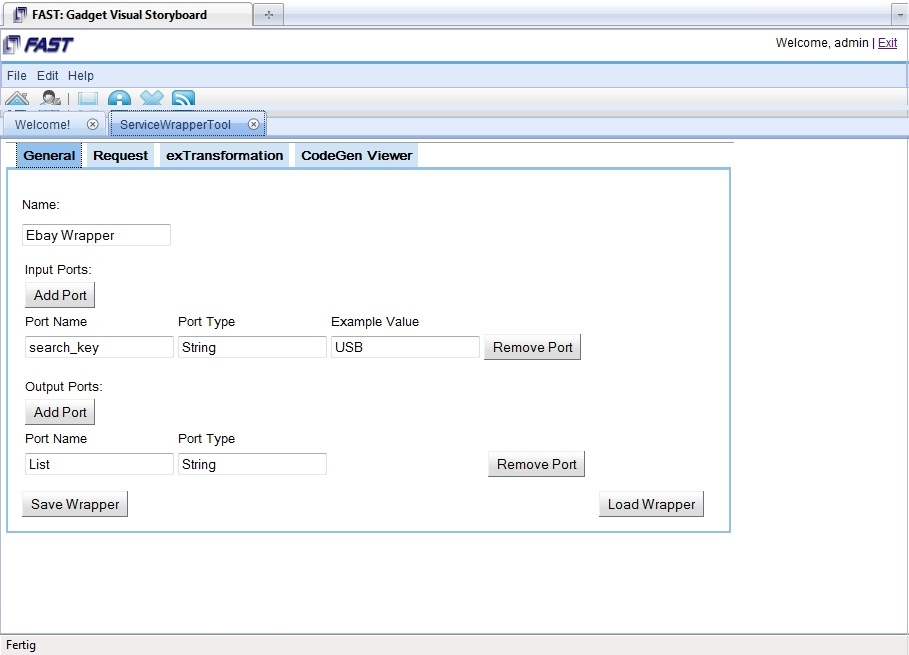
\includegraphics[width=\linewidth]{images/ServiceWrapperToolGVSWithPortDefinitions.jpg}
%    \caption{Configuring parameters of a service wrapper (photoshoped screen dump)}
%    \label{fig:construct_pre_post_conditions}
%  \end{center}
%\end{figure}

The service wrapper tool composes the request using a template string which will contain placeholders for input values. Before sending the request to the service, the placeholders are replaced with their corresponding values and the resulting URL is then ready to be sent as the service request.

Figure ~\ref{fig:construct_service_request} shows the web based tool to construct the service requests.

%\begin{figure}
%  \begin{center}
%    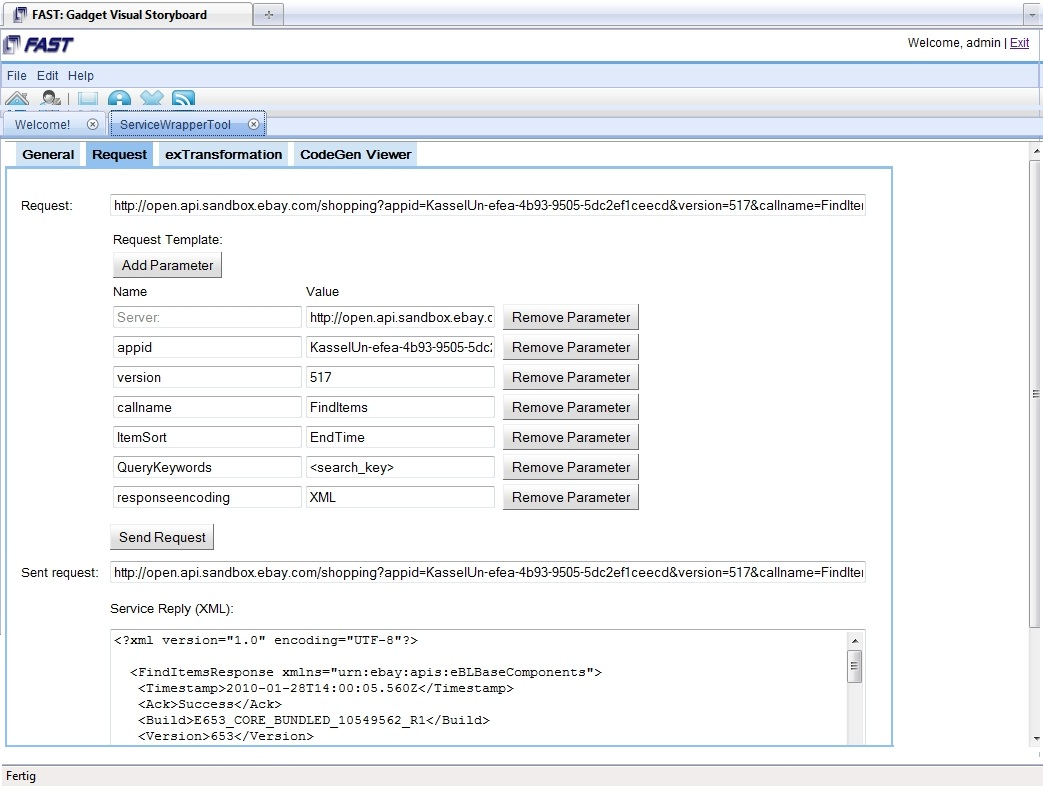
\includegraphics[width=\linewidth]{images/ServiceWrapperToolGVSWithRequestExample.jpg}
%    \caption{Constructing the service request URL and its parameters (photoshoped screen dump)}
%    \label{fig:construct_service_request}
%  \end{center}
%\end{figure}

In the top input field of Figure ~\ref{fig:construct_service_request}, the user may drop an example http request taken e.g. form the service documentation e.g. from \cite{eBayShoppingAPIs}. The tool analyses the example request and in the middle of the screen a form for editing the request parameters is provided. In our example, the user has connected the \textit{QueryKeywords} parameter with the input parameter \textit{search\_key} by adding a corresponding reference to the value field of that parameter. In addition, we have retrieved an access key which has been entered as value for the \textit{appid} parameter.

Below the request parameter editing form of Figure ~\ref{fig:construct_service_request}, a \textit{Send Request} button allows to validate the constructed URL by sending it to the specified service address (via a server relay). Then the placeholders for input parameters are replaced by their example values and the resulting http request is shown below the parameter form. In addition, the request is send and the response is shown on the bottom of that page. This gives the user a fast feedback whether the constructed request works as desired. 

\subsubsection{Limitations} % (fold)
\label{ssub:limitations}



It is worth pointing out that currently the wrapper tool is able to construct input ports for the wrappers using just basic types. To construct URL requests from more complex input parameters, as e.g. a person object, we are currently developing access operations that will allow to access the values of fields of complex objects. For example, the expression \emph{customer.address} may refer to the \emph{address} field of a \emph{customer} parameter.  

% subsubsection limitations (end)

% subsection constructing_service_requests (end)

\subsection{Interpreting service responses} % (fold)
\label{sub:interpreting_service_responses}

Once the service request is constructed and sent to the service provider, it will send back a response. This response message could be serialized in any format, though the most common formats used nowadays are XML or JSON among others. To continue the example started in the previous section, the response of the Ebay Shopping service will be in XML as specified in the request.

\subsubsection{Translation XML into Facts} % (fold)
\label{ssub:translation_xml_into_facts}

Figure ~\ref{fig:response_service_execution} shows the data transformation tab of the wrapper tool. 

%\begin{figure}
%  \begin{center}
%      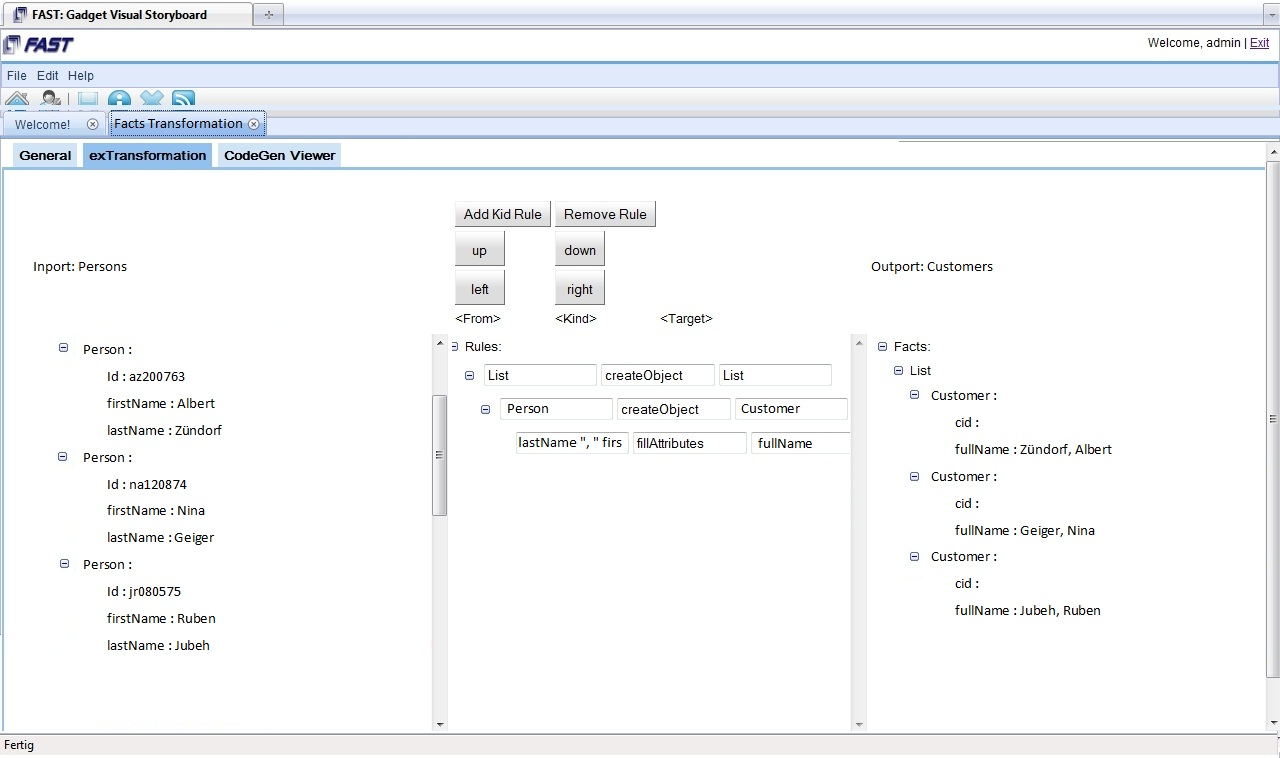
\includegraphics[angle=90,width=0.8\linewidth]{images/ServiceWrapperToolGVSWithTransformationRules.jpg}
%    \caption{Interactive, rule based transforming of an XML response to domain objects (photoshoped screen %dump)}
%    \label{fig:response_service_execution}
%  \end{center}
%\end{figure}

Once the service response, in XML format, has been retrieved, the transformation tab shows it as an interactive object tree on the left side of Figure ~\ref{fig:response_service_execution}. To construct this interactive object tree, the XML document has been parsed into a DOM, and a simplified tree representation of that DOM is built up. 

A transformation rule is used to analyze the XML data and to generate domain-specific objects from concepts from the ontologies used by the parameters of the different building blocks. A transformation rule is composed of three elements, cf. the middle part of Figure ~\ref{fig:response_service_execution}. First, the \textit{from} field indicates the XML elements to be translated by the rule. These XML elements are identified by the tag name of a DOM element from the XML document. Second, the type of the rule will be set, taking one of the following values: \emph{createObject}, \emph{fillAttributes} or \emph{dummy}. And third, the target of the rule specifies a certain concept or attribute, to be created or filled. A detailed explanation of the type of actions to be trigger from the transformation rules is:
\begin{description}
	\item[action \emph{createObject}] specifies the creation of a new domain object. The type of that new object is provided in the third compartment. In the example being explained, the root rule searches for XML elements with tag name \emph{FindItemsResponse} and for each such element a \emph{List} object is created. The resulting objects are shown in a facts tree in the right of Figure ~\ref{fig:response_service_execution}.
	\item[action \emph{fillAttributes}] does not create a new object but it fills the value of the attribute provided as third part of such rules. In our example, the third transformation rule searches for XML elements with tag name \emph{Title}. Note, the rule is a sub-rule of the second rule, which generates \emph{Product} objects. Thus, the sub-rule searches for \emph{Title} tags only in the subtree of the XML data that has been identified by an application of the parent rule before. For example, the \emph{Item} rule may just have been applied to the first \emph{Item} element of the XML data. Then, the \emph{Title} rule is applied only to the first \emph{Item} sub-tree of the XML data and thus it will find only one \emph{Title} element in that sub-tree (not visible in Figure ~\ref{fig:response_service_execution} ). The value of that \emph{Title} element is then transfered to the \emph{productName} attribute of the corresponding \emph{Product} object. Actually, our \textit{from} fields allows also to refer to parts of an XML attribute e.g. to \textit{words} 1 through 3. It is also possible to combine constant text and elements of multiple XML tree elements. 
	\item[action \emph{dummy}] does not create or modify any objects but such rules are just used to narrow the search space for their sub-rules. For example, in Amazon product data, the XML data for an item contains sections for \emph{minimum price}, \emph{maximum price}, and \emph{average price}. Each such section contains the \emph{plain price} and the \emph{formatted price}. Thus, in the Amazon case, a rule that searches for \emph{formatted price} elements within an \emph{Item} element would retrieve three matches. Using a dummy rule, we may first search for \emph{minimum price} elements and then search for \emph{formatted price} elements within that sub-tree.
\end{description}

Our tool follows an interactive paradigm. Therefore, any time a change to a transformation rule is done, the transformation process is triggered and the resulting facts tree is directly shown. This process helps the user to deal with the slightly complex semantics of the transformation rules avoiding errors or mistakes. In addition, out tool is ontology-driven, therefore, the service wrapper designer shall retrieve the domain-specific types from a FAST ontology server together with the structure of each type, i.e. together with a description of the attributes of each object. Thus, the transformation rule editor is able to provide selection boxes for the target element of the rules. For a \emph{createObject} rule, this selection box shows the object types available for that domain. For the \emph{fillAttributes} rules, the selection box shows the attributes of the object type chosen in the parent rule. In addition, we may provide some analysis tool, which will help to guarantee that the objects generated by the transformation rules conform to the object types defined in the corresponding FAST ontology. This helps to ensure that the objects generated by the designed service wrapper will be compatible for input parameters of subsequent filter steps and or gadgets.

% subsubsection translation_xml_into_facts (end)

% subsection interpreting_service_responses (end)

\subsection{Generating a Resource Adapter} % (fold)
\label{sub:generating_a_resource_adapter}

Once the wrapping of a service has been defined and tested in the service wrapper tool, we generate an implementation of the desired Resource Adapter in XML, HTML, and JavaScript, ready to be deployed and executed inside a web gadget. 

% subsection generating_a_resource_adapter (end)

\subsection{Limitations} % (fold)
\label{sub:limitations}

The rule driven approach presented above is somewhat limited. It is deliberately restricted to such a simple rule mechanism in order to keep things simple enough for end-users. Still, the selected approach suffices for many practical and real world cases. As a more complex example, the XML data for a person may provide two different tags for the first and the last name of a person. Contrarily, a person fact which conforms to a certain ontology for that domain may provide only one \emph{fullname} attribute that shall be filled by a concatenation of the first and the last name. To achieve this, the \textit{from} field of that tranforamtion rule might look like: \texttt{lastname"', "`firstname}. We are also able to do some navigation in the XML tree to follow XRef elements. For example the attribute \texttt{grandmother} could be filled using \texttt{mother.mother} in the \textit{from} field. 

However, there are some transformations that these rules cannot perform. For example, we do not support any mathematical operations. Thus, transforming e.g. Fahrenheit into Celsius temperatures is not supported. To cover such  cases, intermediate object formats can be used which would allow generating objects to be further processed by additional filters. Such additional filters may be realized using (hand coded) operators, since some generic operators can act as filters for aggregation and conversions of objects from multiple sources. Then, service wrappers in combination with these filter operators will allow covering these complex cases.

% subsection limitations (end)

% section restful_web_services_wrapper_tool (end)


\section{Discovery: the marketplace}
\label{sec:discovery}

The area of web service publication and discovery has been subject for a lot of research since the very beginning the concept was coined. The current state of the art provides several solutions and strategies which providers and consumers may take advantage of. However, as explained in previous sections, a large number of them suffer from limitated syntactic-based descriptions and a simple keyword-based search, and the gap between discovery and consumption is an obstacle for their usage by a non-technical common user. In order to ligthen the issue, this paper presents yet another publishing platform, permiting any enterprise or individual to publish their public domain web services, with an enhanced semantic search based on the definition of the services, and serving``web service wrappers'' for easily consumption in any web application.

\subsection{Overview}
\label{ssec:overview}

The main difference of this platform with regards to the state of the art is that it is clearly targeting a different kind of user, and covers many deficiencies others tools does not tackle with. As a briefly overview, the platform being presented:

\begin{itemize}
	\item offers web services as Linked Data;
	\item serves web services wrappers ready-to-consume in any web application;
	\item follows well-known best practices for publishing data on the web;
	\item supports managing its resources via its RESTful API;
	\item supports content negotiation so the different clients may retrieved the information in JSON, RDF/XML, RDF/N3 or a human-readable HTML version;
	\item provices advanced search capabilites, based on the service formal definition and inferences extracted from it;
	\item a SPARQL endpoint to access directly to the data allowing advanced queries;
\end{itemize}

This platform was intented and it is being used as part of the FAST storyboard tool. Others components communicates with it via its RESTful API, but a
That said, The process of publishing a web service requires two steps: (i) generation of the wrapper (see Sec. \ref{sec:wrapping_web_services}, and (ii) creation of the resource in the publishing platform. The creation of the resources is done via the public RESTful API, and the language selected for the input for any operation is JSON. The following is an example of part of a request sent to create a new wrapper into the platform:

\begin{listing}
\begin{verbatim}
{
  "code": "http://demo.fast.morfeo-project.org/code/amazonService.js",
  "creationDate": "2010-01-26T17:01:13+0000",
  "description": {"en-gb": "Amazon web service"},
  "label": {"en-gb": "Amazon web service"},
  "preconditions": [
    [
      {
        "id": "item",
        "label": { "en-gb": "An item" },
        "pattern": "?I http://www.w3.org/1999/02/22-rdf-syntax-ns#type http://aws.amazon.com/AWSECommerceService#Item",
        "positive": "true"
      }
    ]
  ],
  "postconditions": [
    ...
  ],
  ...
\end{verbatim}
\label{lis:json_request}
\end{listing}

The architecture, as presented in the Figure \ref{fig:}, comprises a RDF store used for persistence, a business layer dealing with the model and reasoning, and public fa�ade providing the core functionality as a RESTful API, and a SPARQL endpoint accessing directly the RDF store. This presentation layer is aimed to interact with the FAST Gadget Visual Storyboard, or any other third-party application.

The RESTful API and the SPARQL endpoint are part of the presentation layer. The SPARQL endpoint is offered using the SPARQL protocol service as defined in the SPROT specification \cite{sprot} and is aimed to enable third-party developers to query directly the knowledge base using SPARQL queries. This feature is supported by the Sesame RESTful HTTP interface for SPARQL Protocol for RDF.

The business logic layer contains all the domain-specific processing and reasoning. It provides functions to interact with all the elements of the domain model specified in \cite{sec:model}, acting as a mediator between the public RESTful API and the persistence layer.

The persistence layer provides an API to work with a standard set of objects representing the model. The interaction with the underlying RDF store is made via RDF2Go, an abstraction over triple (and quad) stores, which allows to program against rdf2go interfaces and choose any the RDF store implementation. This allows having a completely extensible and configurable framework for storage mechanisms, inferencers, RDF file formats, query result formats and query languages...

How to publish (RESTful app, anyone can create a wrapper and publish it)

How to browse: will allow users to go through the given domains (ontologies) and concepts, and will explain how to find the services they want (operation Find of the catalogue) => how the recommendation/reasoning works



It offers the wrapped web services as linked data and has an open sparql endpoint, allowing other developers to create applications on top of it...

\subsection{Serving Linked Data} % (fold)
\label{sub:linked_data}

The recently success of the web of Data has influenced the way information is now published on the web, and has been widely adopted by the academic community, large companies such as The New York Times and BBC, and national governments such as US and UK made public commitments toward open data. The main aim of the linking data is to find other related data based upon previously known data, in terms of the connections or links between them. We apply this concept in order to provide metadata about the web services as linked data, following the principles as originally defined in \cite{bizer_ijswis2009}, in order to make them available to arbitrary third-party applications. Each web service is identified by an HTTP URI and hosted in the catalogue so that it can be dereferenced through the same URI. For each building block, data is available in representations in different standard formats such as JSON (for communication with the GVS), RDF/XML, Turtle, or even HTML+RDFa as a human-readable version. The principles and best practices proposed in \cite{berrueta2008} and \cite{sauermann2008cool_uris} are also taken into account, these representations are served based on the request issued by the requesting agent, using a technique called \emph{content negotiation}. As required by the forth rule of linked data, individual building blocks link to other data on the web, thereby preventing so-called isolated ``data islands''.

In order to understand how content negotiation is implemented in the catalogue, a few concepts need to be understood. The URI of a particular building block must be understood as the identifier of the building block as such, as opposed to a particular representation (JSON, HTML, etc.) of it. In fact, each such representation has its own URI, under which it can be retrieved. Using the terminology established in \cite{w3c2004webArchitecture}, the building block is a \emph{non-information resource}, whereas each representation is an \emph{information resource}. In the process of content negotiation, the requesting agent will first request the URI of the building block as such (e.g., \texttt{http://catalogue.com/screens/235}), as well as the required representation format (e.g., JSON). The catalogue will then inspect the request and redirect the requester to the appropriate representation (e.g., \texttt{http://catalogue.com/screens/235.json}), as illustrated in Fig.~\ref{fig:content_negotiation}.
On the web, different representations for the same resource are called \emph{variants}, and content negotiation is the mechanism used to determine which of the representations of most appropriate for a given request.

%\begin{figure}[htb]
%\label{fig:content_negotiation}
%\begin{center}
%	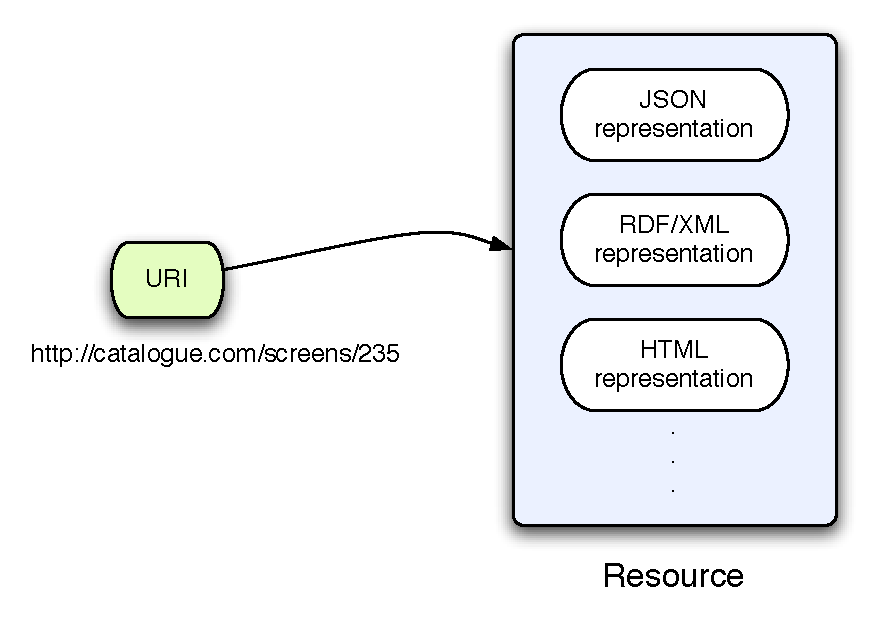
\includegraphics[width=12cm]{images/content_negotiation}
%	\caption{Content Negotiation}
%\end{center}
%\end{figure}

In summary, the basic idea of content negotiation, as stated in the \cite{http1.1}, is to serve the best variant for a resource, taking into account what variants are available, what variants the server may prefer to serve, what the client can accept, and with which preferences. In HTTP, this is done by the client which may send, in its request, accept headers (\texttt{Accept}, \texttt{Accept-Language} and \texttt{Accept-Encoding}), to communicate its capabilities and preferences in format, language and encoding, respectively.

In fact, what the catalogue really does is ``format negotiation'' since the alternate representations are just based on the selection of the media type, through the accept header, but does not consider different languages or encoding types. The formats supported are JSON, RDF/XML, Turtle and HTML+RDFa. Even though the accept header is desired, the different representations can also be retrieved directly by dereferencing their own URI. The convention used in the catalogue for deriving a representation URI from a building block URI is to simply attach a matching suffix, such as \texttt{.rdf}, \texttt{.json} or \texttt{.html}.

Lastly, content negotiation needs to identify which player is going to take the lead on it. There are two kinds of content negotiation which are possible in HTTP: server-driven and agent-driven negotiation. The approach followed by the catalogue is agent-driven negotiation, hence selecting a specific representation for a resource is responsibility of the user agent. If none is specified, by default, the server will choose the JSON representation.


\subsection{Simplified Model/Ontology (Knud)}
The model used to define the web service wrappers within this application has been influenced by WSDL, the main web service definition language, and some semantic-enriched approaches such as WSMO and OWL-S. There is no need to reinvent the wheel, 

A WSDL operation is mapped to an action. Its inputs and outputs are called pre-postconditions (a WSMO concept). 

This section could talk about a the part of the ontology describing the back-end services, how we remove the unnecessary information from WSDL and similar (not need anymore because the code has been generated), however we reuse some of the concepts from these technologies to define them (preconditions, postconditions, actions, and so on) allowing discovery and composition.

%\begin{figure}[ht]
%	\centering
%	\includegraphics[width=8.31cm]{uddi.png}
%	\caption{UDDI overview}
%	\label{fig:uddi}
%\end{figure}


%\section{Wrapping web services (Kassel)}
%\label{sec:wrapping_web_services}

%This section talks about the service wrapper tool (Kassel prototype)

%What it offers

%How to create a wrapper (test-and-construct approach)

%Place this component within the FAST architecture

%Talk about formats: JSON and XML??


%\subsection{Code-generation phase}
%How the executable code is build:

% - mapping from operations and parameters to actions and preconditions

% - mapping from operation results to postconditions

%Now, the calls are done through the FAST api, which acts as a proxy <- imply they need to construct the widget using the FAST GVS which doesn't give an open solution (proposal in future work)


\section{Use case}
maybe we should provide some kind of use case to show the benefits of the approach and the possibilities this sort of tools?

\section{Conclusions and future work}

Future work:

Talk about wrapping WSDL-based services

Talk about WSMO-lite services

Use JSONRequest to replace the AJAX XMLHttpRequest and its problems (cross-domain calls), so there's no need for a Proxy.

\subsubsection*{Acknowledgments.} This work is supported in part by the European Commission
under the first call of its Seventh Framework Program (FAST STREP Project, grant
INFSO-ICT-216048) and in part by Science Foundation Ireland under Grant No.
SFI/08/CE/I1380 (L\'ion-2).


\bibliographystyle{apalike}
\bibliography{paper}


\section*{Checklist of Items to be Sent to Volume Editors}
Here is a checklist of everything the volume editor requires from you:


\begin{itemize}
\settowidth{\leftmargin}{{\Large$\square$}}\advance\leftmargin\labelsep
\itemsep8pt\relax
\renewcommand\labelitemi{{\lower1.5pt\hbox{\Large$\square$}}}

\item The final \LaTeX{} source files
\item A final PDF file
\item A copyright form, signed by one author on behalf of all of the
authors of the paper.
\item A readme giving the name and email address of the
corresponding author.
\end{itemize}
\end{document}
